%& C:\Users\RANGAR~1\AppData\Roaming\TikzEdt\TikzEdt\023~1.0\TEMP_H~1
\begin{document}
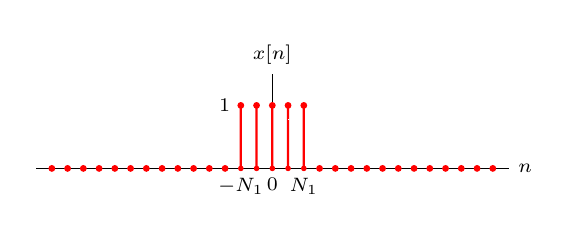
\begin{tikzpicture}[scale=0.8]

	\def\nmin{-13}
	\def\nmax{13}	
	
	\begin{scope}	
		\def\x{{0, 0, 0, 0, 0, 0, 0, 0, 0, 0, 0, 0, 1, 1, 1, 1, 1, 0, 0, 0, 0, 0, 0, 0, 0, 0, 0, 0, 0}}	

		\draw (-3.5, 0) -- (4, 0) node[anchor=west] {\scriptsize $n$};
		\draw (0.25,0) -- ++(0, 1.5) node [anchor=south] {\scriptsize $x[n]$};
		\foreach \n/\l in {-1/{-N_1}, 1/0, 3/{N_1}}
		{
			\node at (\n/4, 0) [anchor=north] {\scriptsize $\l$};
		}
		\node at (-0.75,1) [anchor=west] {\scriptsize $1$};

		
		\foreach \n in {0,1, ..., 28}
		{
			\pgfmathparse{\x[\n]}
			\edef\xn{\pgfmathresult}	
			\ifthenelse{\xn > 0}
			{
				\draw[red, thick, fill=red]  (\n/4 + \nmin/4, 0) -- ++(0, \xn) circle (1pt);% node[anchor=east] {\scriptsize $\xn$};
			}
			{
				\draw[red, fill=red] (\n/4+ \nmin/4,  0) circle (1pt);
			}
		}
	\end{scope}	

\usetikzlibrary{calc}
\pgftransformreset
\node[inner sep=0pt,outer sep=0pt,minimum size=0pt,line width=0pt,text width=0pt,text height=0pt] at (current bounding box) {};
%add border to avoid cropping by pdflibnet
\foreach \border in {0.1}
  \useasboundingbox (current bounding box.south west)+(-\border,-\border) rectangle (current bounding box.north east)+(\border,\border);
\newwrite\metadatafile
\immediate\openout\metadatafile=\jobname_BB.txt
\path
  let
    \p1=(current bounding box.south west),
    \p2=(current bounding box.north east)
  in
  node[inner sep=0pt,outer sep=0pt,minimum size=0pt,line width=0pt,text width=0pt,text height=0pt,draw=white] at (current bounding box) {
\immediate\write\metadatafile{\p1,\p2}
};
\immediate\closeout\metadatafile
\end{tikzpicture}

\end{document}


\end{document}


ent}

cument}

